\documentclass{article}
\usepackage[utf8]{inputenc}  % UTF-8 인코딩 지원
\usepackage[a4paper, margin=1in]{geometry}  % 페이지 여백 설정
\usepackage{titlesec}  % 제목 스타일 조정 패키지
\usepackage{titling}   % 제목 추가 스타일링 지원
\usepackage{graphicx}  % 그래픽 삽입을 위한 패키지
\usepackage{caption}   % 캡션을 위한 패키지
\usepackage{subcaption} % 서브캡션 사용을 위한 패키지
\usepackage{array}     % 표 스타일 조정을 위한 패키지
\usepackage{booktabs}  % 더 좋은 표 스타일을 위한 패키지

% 제목 스타일 조정
\pretitle{\begin{center}\LARGE\bfseries}  % 제목 크기와 굵기 (줄임)
\posttitle{\par\vskip 1em\hrule\vskip 1em\end{center}}  % 제목 아래 라인 추가
\preauthor{\begin{center}\normalsize}  % 작성자 정보 크기 조정
\postauthor{\par\end{center}}
\predate{\begin{center}\itshape}  % 날짜 스타일 조정
\postdate{\par\end{center}}

\title{\textbf{\MakeUppercase{Impact of Data Transformations on Model Accuracy:}\\ \MakeUppercase{Homography and Gaussian Noise}}}  % 제목을 대문자로 변경
\author{
    Minwon Lee \\  % 이름
    Department of Automotive Engineering \\  % 학과명
    Hanyang University \\  % 대학명
    Seoul, South Korea  % 위치
}
\date{\textit{\MakeUppercase{December 6, 2024}}}  % 날짜 대문자

\begin{document}

\maketitle  % 제목, 작성자, 날짜 출력

\begin{abstract}  
    This report evaluates the robustness of various machine learning models, 
    including Logistic Regression, SVM, MLP, and CNN, under two types of data transformations: Homography and Gaussian Noise. 
    In autonomous driving perception systems, such transformations are the most common distortions encountered when recognizing numbers in road images.
    The results highlight model performance differences considering accuracy and suggest considerations for robust machine learning applications. 
\end{abstract}

\section{Problem Setting}
The problem at hand is to evaluate the robustness of several machine learning models when faced with data transformations such as Homography and Gaussian Noise. The objective is to test how well models like Logistic Regression, FDA, SVM, MLP, and CNN perform under these challenging conditions, and to analyze the trade-offs between different models' ability to handle such transformations.

The models will be tested on the MNIST dataset. Before applying any transformations, the **baseline performance** of each model will be evaluated on the original (untouched) data to establish a reference point. This will allow us to compare how much the transformations affect the performance of each model.

\section{Dataset and Data Split}

\subsection{Dataset Overview}
The dataset used for this study contains 1,797 samples, each represented by 64 features. This dataset consists of numerical data derived from handwritten digits. The dataset is uniformly distributed across 10 unique classes, representing digits from 0 to 9. This uniform distribution ensures that each class has roughly the same number of samples, which contributes to a balanced training process.

The dataset is split into training and test sets, with 1,437 samples used for training and 360 samples used for testing. This split ensures that the model can be evaluated on data it has not seen during the training phase.

\begin{figure}[h]
    \centering
    \begin{subfigure}[b]{0.45\textwidth}
        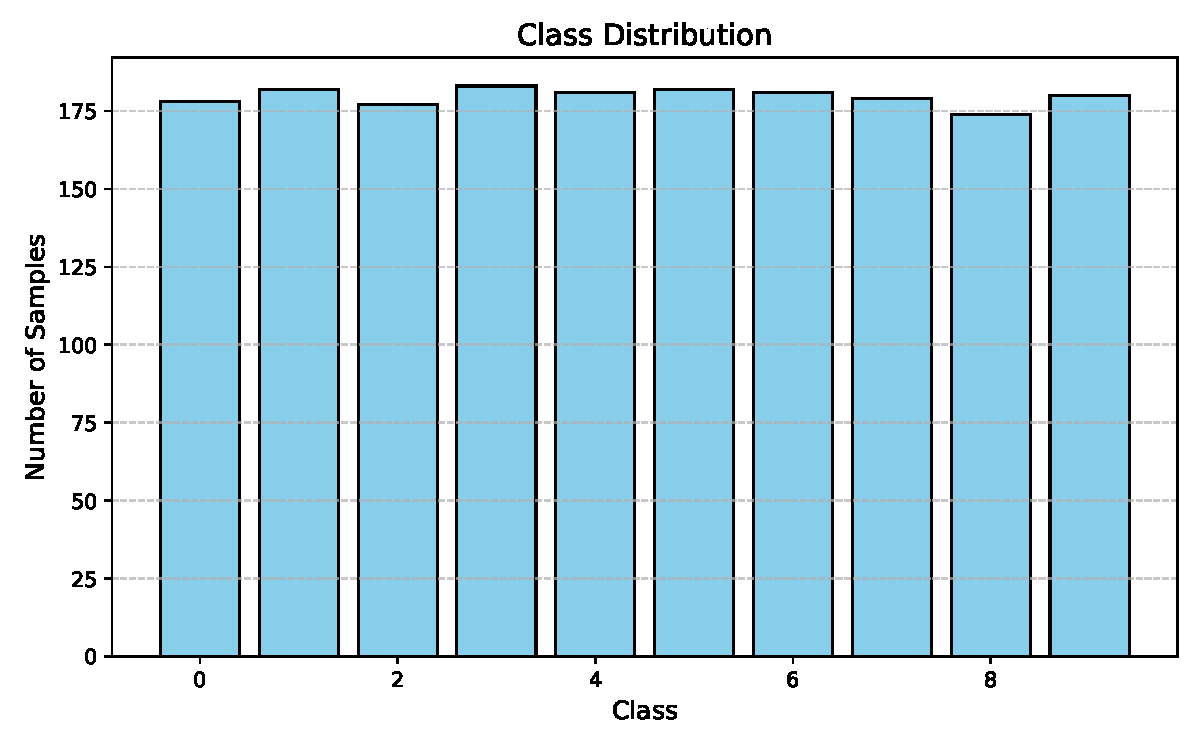
\includegraphics[width=\textwidth]{images/class_distribution.pdf}
        \caption{Class Distribution Visualization}
        \label{fig:class_distribution}
    \end{subfigure}
    \hfill
    \begin{subfigure}[b]{0.45\textwidth}
        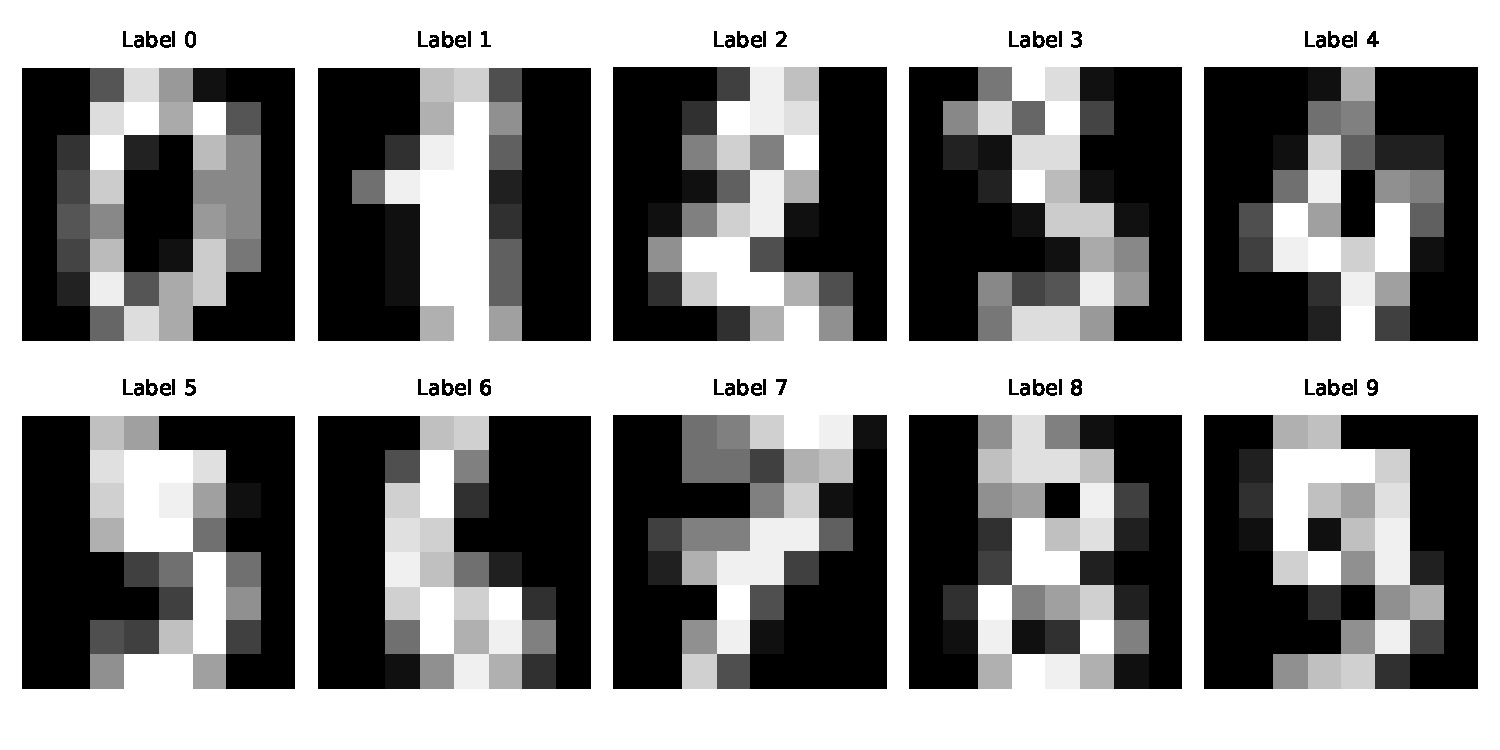
\includegraphics[width=\textwidth]{images/MNIST_samples.pdf}
        \caption{Sample MNIST Images}
        \label{fig:mnist_samples}
    \end{subfigure}
    \caption{Dataset Visualizations: Class distribution and example MNIST images.}
    \label{fig:dataset_visualizations}
\end{figure}

\subsection{Data Split}
The dataset is split into training and test sets. The training set contains 1,437 samples, while the test set consists of 360 samples. The test set is reserved for evaluating the generalization performance of the trained model.

\subsubsection{Train and Validation Split with K-Fold Cross-Validation}
To evaluate the robustness of the model and avoid overfitting, we employ 5-fold cross-validation on the training set. In 5-fold cross-validation, the training data is divided into 5 subsets (folds). The model is trained on 4 folds and validated on the remaining fold, and this process is repeated 5 times, with each fold serving as the validation set once.

The details of the data split for each fold are as follows:

\begin{itemize}
    \item \textbf{Fold 1}: Training indices: 1,149; Validation indices: 288
    \item \textbf{Fold 2}: Training indices: 1,149; Validation indices: 288
    \item \textbf{Fold 3}: Training indices: 1,150; Validation indices: 287
    \item \textbf{Fold 4}: Training indices: 1,150; Validation indices: 287
    \item \textbf{Fold 5}: Training indices: 1,150; Validation indices: 287
\end{itemize}

\section{Models and Validation Accuracy}

\subsection{Model Overview}
The following machine learning models are used in this study to evaluate their robustness against data transformations:

\begin{itemize}
    \item \textbf{Logistic Regression}: A linear model used for binary and multi-class classification, employing the logistic function to predict class probabilities.
    \item \textbf{Fisher Discriminant Analysis (FDA)}: A linear discriminant analysis model used to project data in such a way that maximizes class separability.
    \item \textbf{Support Vector Machine (SVM)}: Two versions are used in this study - one with an RBF kernel for non-linear classification and another with a polynomial kernel.
    \item \textbf{Multilayer Perceptron (MLP)}: A simple neural network model with a hidden layer, capable of learning complex non-linear patterns.
    \item \textbf{Convolutional Neural Network (CNN)}: A more advanced deep learning model particularly well-suited for image data.
\end{itemize}

\subsection{Validation Accuracy for Each Model}
The table below summarizes the validation accuracy of each model after performing 5-fold cross-validation on the training set. The values represent the average accuracy across the 5 folds.

\begin{table}[h]
    \centering
    \caption{Average Validation Accuracy for Each Model}
    \label{tab:validation_accuracy}
    \begin{tabular}{l c}
        \toprule
        \textbf{Model} & \textbf{Average Validation Accuracy} \\
        \midrule
        Logistic Regression & 0.9617 \\
        Fisher Discriminant Analysis (FDA) & 0.9478 \\
        SVM (RBF Kernel) & 0.9861 \\
        SVM (Polynomial Kernel) & 0.9882 \\
        Multilayer Perceptron (MLP) & 0.9763 \\
        Convolutional Neural Network (CNN) & 0.9792 \\
        \bottomrule
    \end{tabular}
\end{table}

The 5-fold cross-validation ensures that each data point in the training set is used for both training and validation, which helps provide a more reliable estimate of the model's performance and minimizes bias.

\subsection{Preprocessing and Feature Extraction}
Before training the models, the features are normalized to improve convergence during training. The feature values, originally in the range from 0.0 to 16.0, are scaled to a range of [0, 1] by dividing each value by 16.0. This normalization ensures that all features contribute equally during the training of the model, avoiding dominance by features with larger numerical values.

\section{Experimental Setup}

\subsection{Homography Transformation}
The homography transformation involves altering the perspective of the images to simulate distortions that might occur in real-world scenarios, such as capturing an image at an angle. In this study, we applied a perspective transformation by modifying the coordinates of the four corners of the image. Specifically, each corner's position was adjusted by adding a random offset within a maximum range specified by \textbf{max\_offset}. 

Three different levels of homography transformations were tested:
\begin{itemize}
    \item \textbf{offset = 1.5}: Each corner was shifted by a random value within the range of [-1.5, 1.5] pixels.
    \item \textbf{offset = 2.0}: Each corner was shifted by a random value within the range of [-2.0, 2.0] pixels.
    \item \textbf{offset = 2.5}: Each corner was shifted by a random value within the range of [-2.5, 2.5] pixels.
\end{itemize}

This transformation was intended to test how well each model can handle changes in perspective. The range of offsets was chosen to progressively increase the severity of the transformation, thereby evaluating the robustness of the models under increasingly difficult conditions.

\subsection{Gaussian Noise}
Gaussian noise was added to the images to simulate noisy conditions that are often encountered in real-world image data, such as low-light conditions or sensor noise. Gaussian noise was introduced to the dataset at three different levels, each with a different value of standard deviation (\textbf{sigma}):

\begin{itemize}
    \item \textbf{sigma = 0.2}: A moderate level of Gaussian noise.
    \item \textbf{sigma = 0.5}: An increased level of noise, introducing noticeable degradation in the image quality.
    \item \textbf{sigma = 0.7}: A high level of noise, significantly affecting image clarity and making the classification task more challenging.
\end{itemize}

The objective of introducing Gaussian noise was to evaluate the models' tolerance to noisy data. This is especially important in real-world applications where images are rarely pristine, and the robustness of the model under such conditions is crucial.

\subsection{Transformation Visualization}
To provide a qualitative insight into the applied transformations, Figure~\ref{fig:experiment_visualization} illustrates the impact of Homography (max\_offset = 2.5) and Gaussian Noise (sigma = 0.7) on sample images from the dataset. These examples represent the most challenging transformations applied in this study.

\begin{figure}[h!]
    \centering
    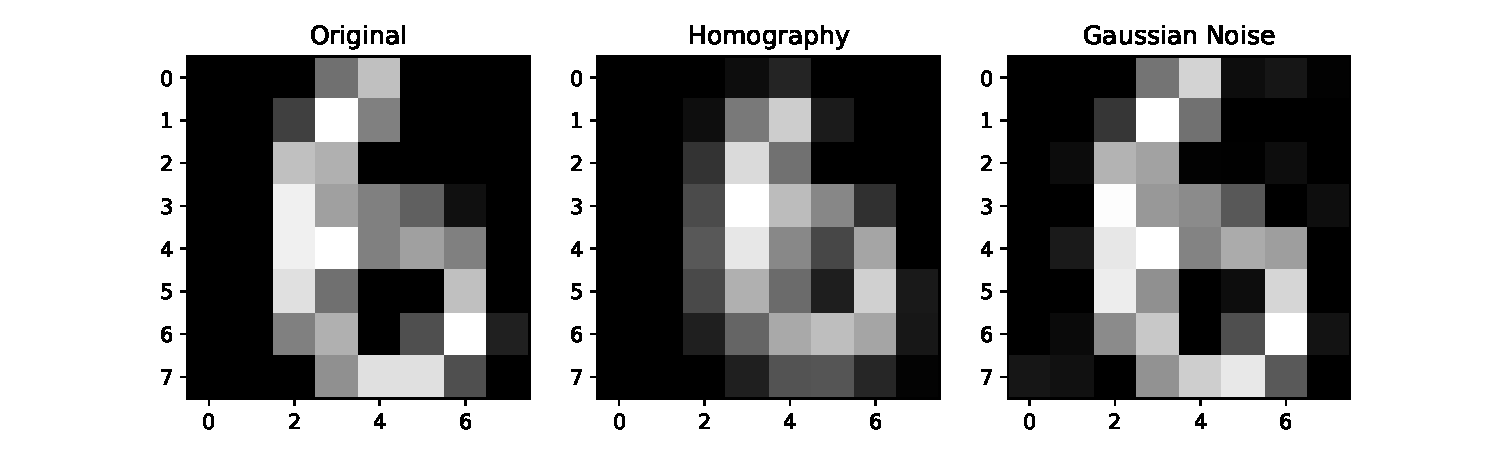
\includegraphics[width=0.8\textwidth]{images/Experiment.pdf}
    \caption{Visualization of Homography Transformation (max\_offset = 2.5) and Gaussian Noise (sigma = 0.7).}
    \label{fig:experiment_visualization}
\end{figure}

\subsection{Model Training and Evaluation}
The models were trained on the original (untouched) training dataset and subsequently evaluated on:
\begin{enumerate}
    \item The original test dataset (Baseline performance).
    \item The homography-transformed datasets with max\_offset values of 1.5, 2.0, and 2.5.
    \item The Gaussian noise-transformed datasets with sigma values of 0.2, 0.5, and 0.7.
\end{enumerate}

Each transformation type was tested at different severity levels, as described above, to understand how the model accuracy changes as the degree of transformation increases. This allowed us to analyze the strengths and weaknesses of each model when subjected to distortions common in autonomous driving environments, such as perspective shifts and noise interference.

\section{Experiment Results}

\subsection{Baseline Accuracy}
The baseline accuracy represents the performance of each model on the original MNIST dataset without any transformations. Figure~\ref{fig:baseline_accuracy} illustrates the baseline accuracy for all models, highlighting the effectiveness of CNN and SVM with a polynomial kernel, which achieved the highest accuracy.

\begin{figure}[h!]
    \centering
    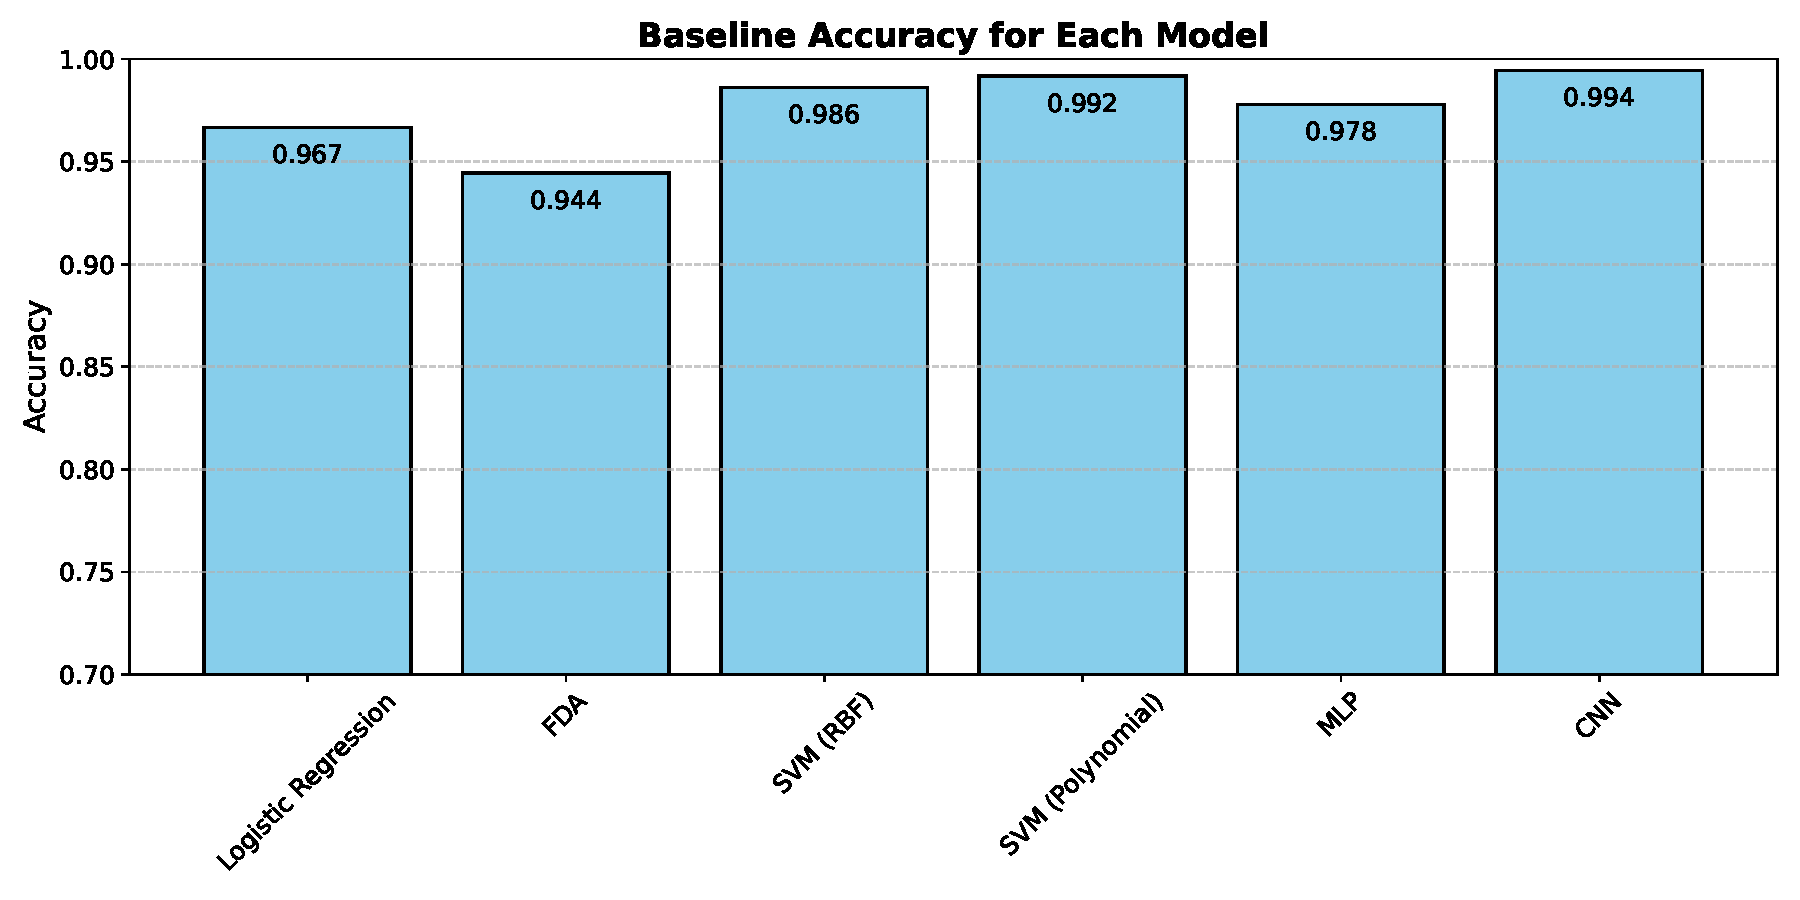
\includegraphics[width=0.8\textwidth]{images/baseline_accuracy.pdf}
    \caption{Baseline accuracy for each model on the original MNIST dataset.}
    \label{fig:baseline_accuracy}
\end{figure}

\subsection{Impact of Homography Transformation}
The robustness of the models was tested by applying homography transformations with varying degrees of severity (max\_offset = 1.5, 2.0, 2.5). As shown in Figure~\ref{fig:homography_accuracy}, the accuracy of all models decreases as the severity of the transformation increases. CNN outperformed other models, demonstrating its ability to handle perspective distortions more effectively.

\begin{figure}[h!]
    \centering
    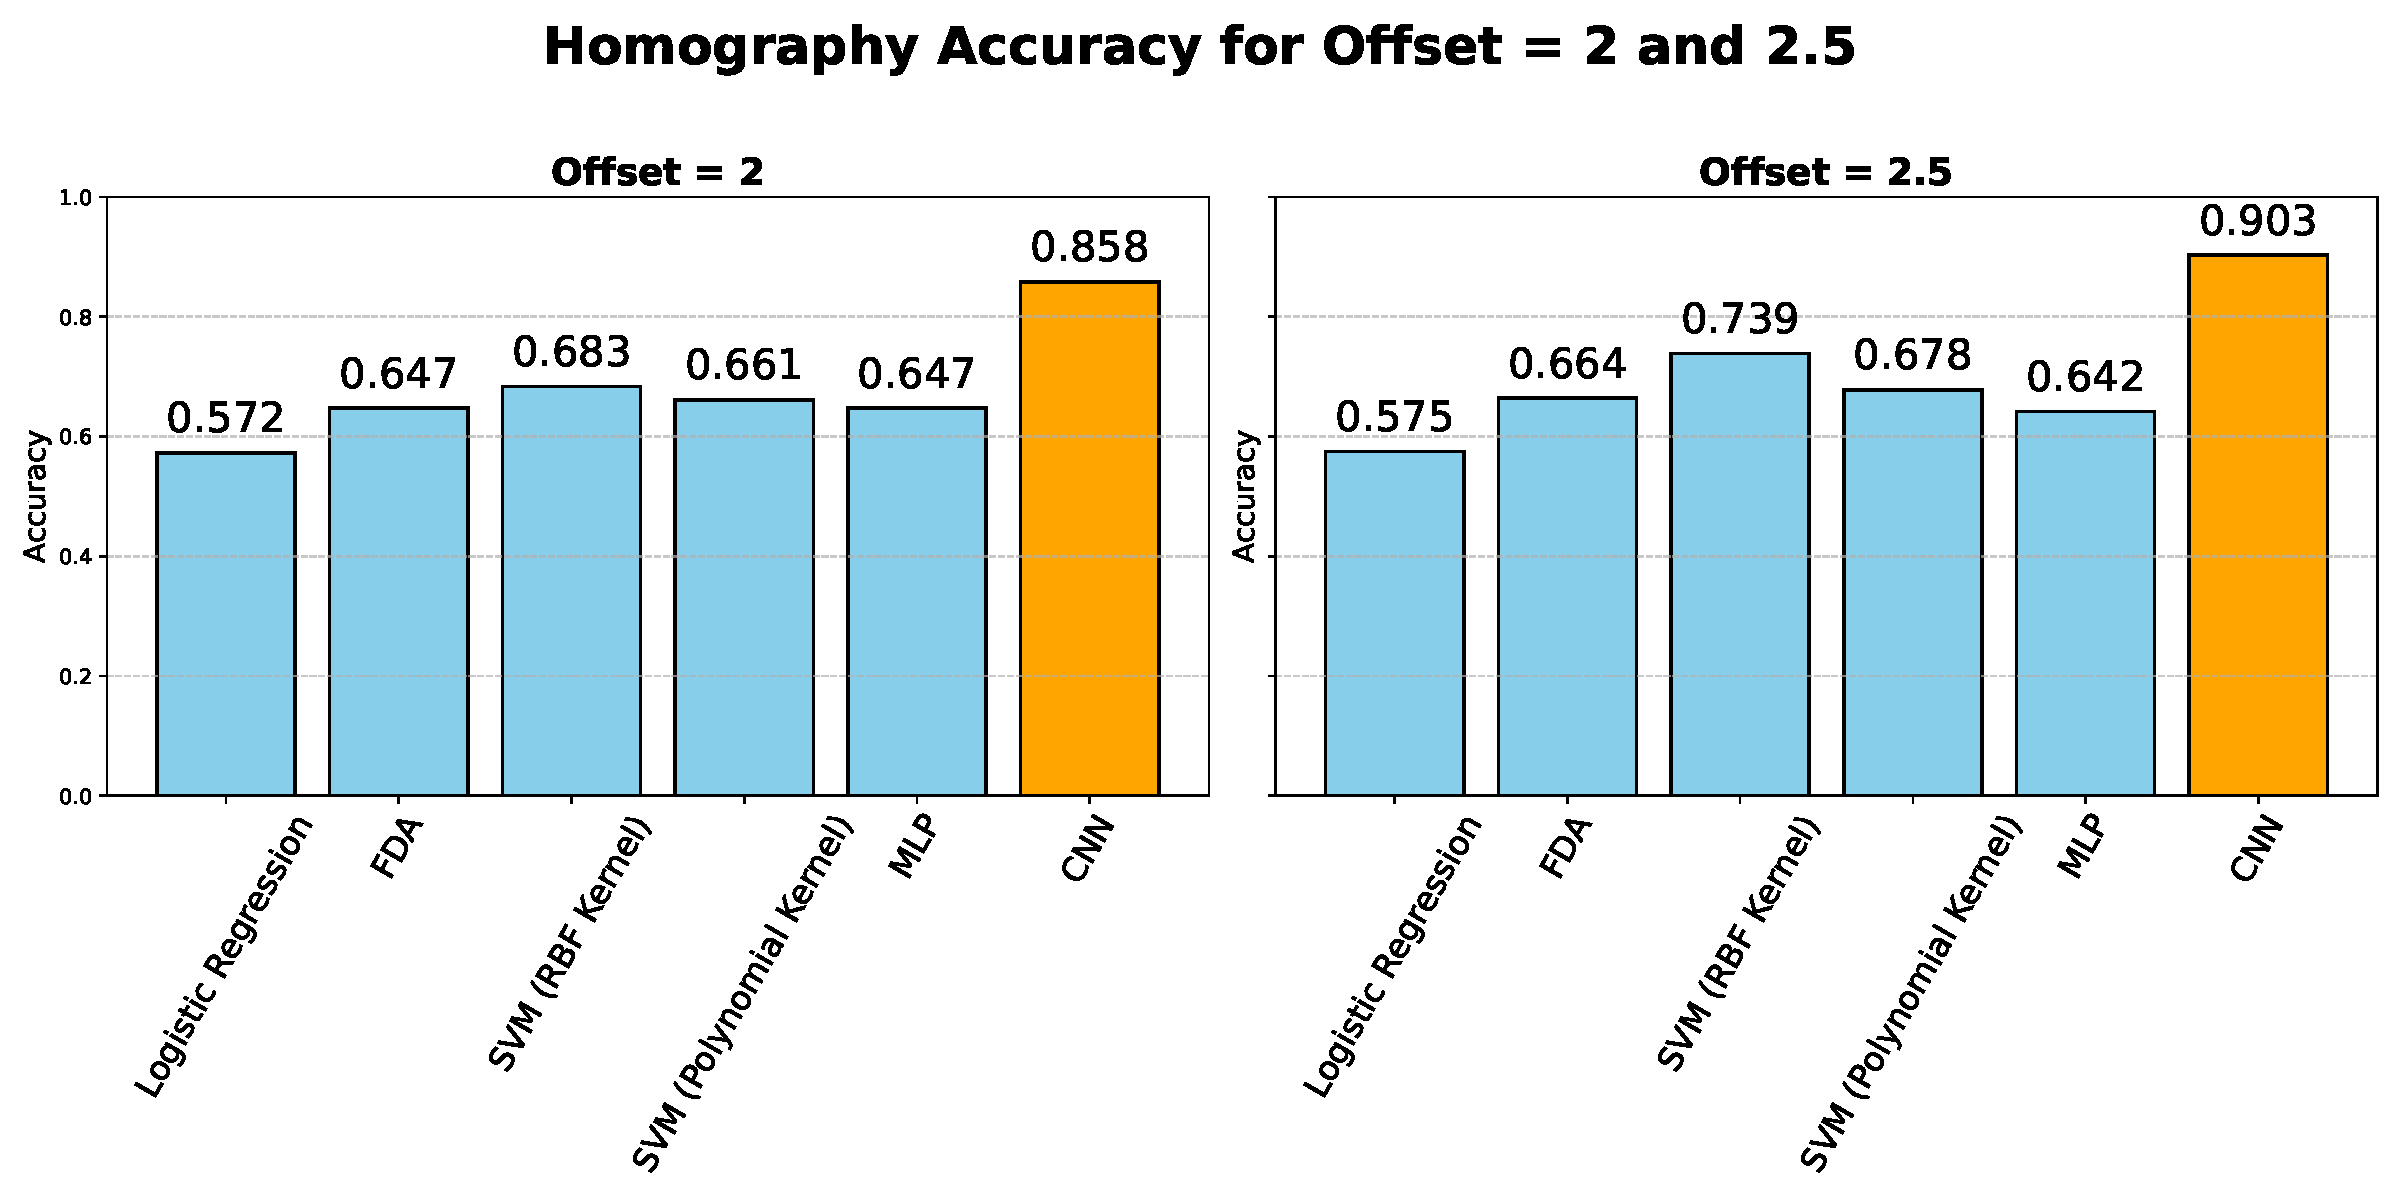
\includegraphics[width=0.8\textwidth]{images/homography.pdf}
    \caption{Accuracy under homography transformations with different max\_offset values.}
    \label{fig:homography_accuracy}
\end{figure}

\subsection{Impact of Gaussian Noise}
Gaussian noise with varying sigma values (0.2, 0.5, 0.7) was added to the test data to simulate noisy environments. The results, presented in Figure~\ref{fig:gaussian_noise_accuracy}, reveal that the models' performance degrades as the noise level increases. However, SVM with a polynomial kernel and CNN demonstrated relatively high tolerance to Gaussian noise.

\begin{figure}[h!]
    \centering
    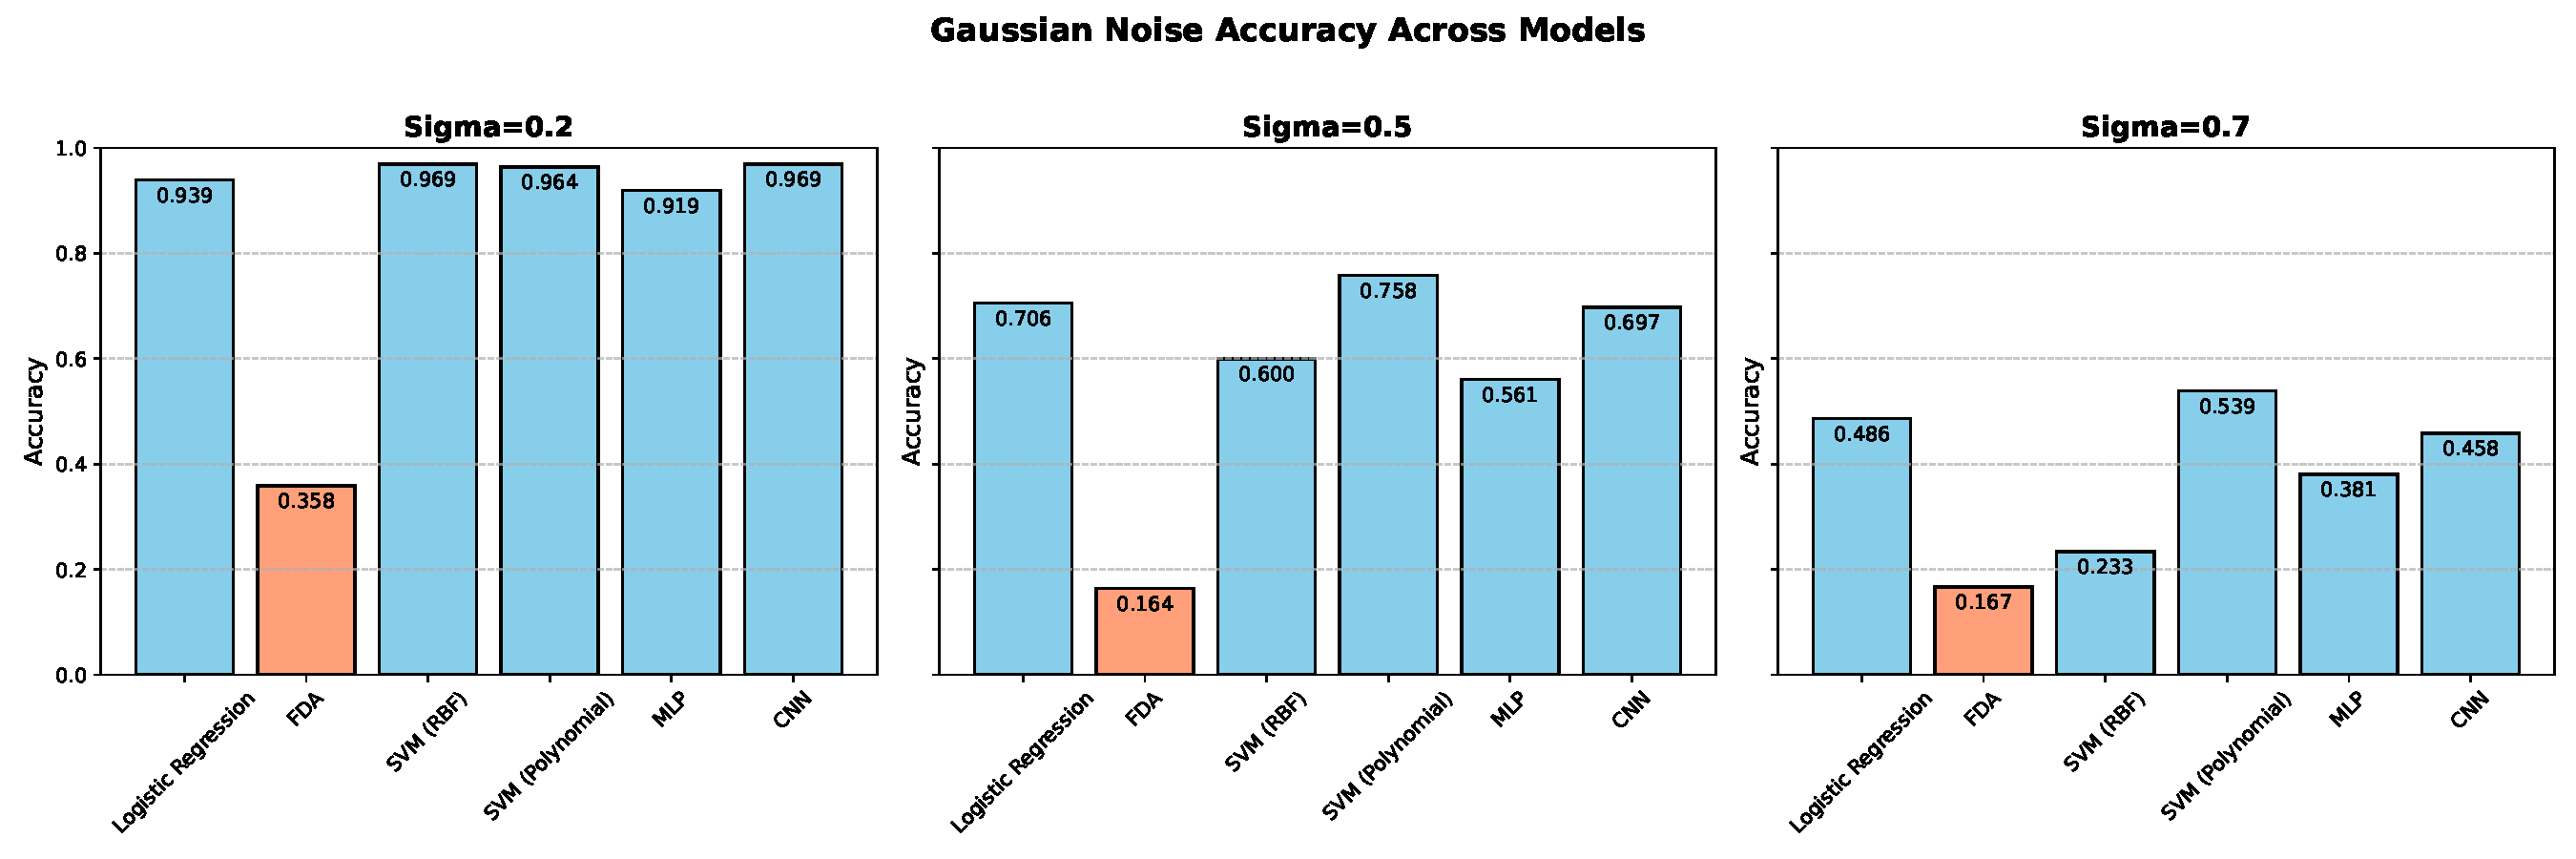
\includegraphics[width=0.8\textwidth]{images/gaussian_noise.pdf}
    \caption{Accuracy under Gaussian noise transformations with different sigma values.}
    \label{fig:gaussian_noise_accuracy}
\end{figure}

\subsection{Analysis and Comparison of Results}

\subsubsection{Brief Explanation of Algorithms}
Each algorithm has unique characteristics that make it suitable for specific tasks:
\begin{itemize}
    \item \textbf{Logistic Regression}: A simple linear classifier effective for baseline evaluations.
    \item \textbf{Fisher Discriminant Analysis (FDA)}: Projects data to maximize class separability but struggles with non-linear boundaries.
    \item \textbf{Support Vector Machine (SVM)}: Excels in finding decision boundaries with kernels for linear and non-linear tasks.
    \item \textbf{Multilayer Perceptron (MLP)}: A basic neural network capable of learning non-linear patterns.
    \item \textbf{Convolutional Neural Network (CNN)}: Best-suited for image-based tasks due to its ability to learn spatial hierarchies.
\end{itemize}

\subsubsection{Performance Analysis for Each Algorithm}
The results reveal that CNN consistently outperforms other models, achieving the highest accuracy under both baseline and transformation scenarios. However, the following patterns were observed:
\begin{itemize}
    \item \textbf{Baseline Accuracy}: CNN and SVM (Polynomial Kernel) delivered the best results, demonstrating their capability to model complex patterns in data.
    \item \textbf{Homography Transformation}: CNN showed higher resilience to perspective shifts, maintaining relatively high accuracy even under severe offsets.
    \item \textbf{Gaussian Noise}: SVM with Polynomial Kernel and CNN were the most robust to noise, maintaining stable accuracy compared to other models.
\end{itemize}

\subsubsection{Comparative Results}
Table~\ref{tab:comparison} provides a summary of the comparative results across all scenarios, showcasing the models' performance under varying conditions. This comparison highlights the trade-offs between linear and non-linear models and demonstrates the superiority of CNN in handling real-world distortions.

\begin{table}[h!]
    \centering
    \caption{Comparative Results for Each Algorithm Across All Scenarios}
    \label{tab:comparison}
    \begin{tabular}{|l|c|c|c|}
        \hline
        \textbf{Model} & \textbf{Baseline Accuracy} & \textbf{Homography (Avg.)} & \textbf{Gaussian Noise (Avg.)} \\
        \hline
        Logistic Regression & 0.9667 & 0.7018 & 0.7102 \\
        FDA & 0.9444 & 0.7417 & 0.2293 \\
        SVM (RBF Kernel) & 0.9861 & 0.7851 & 0.6009 \\
        SVM (Polynomial Kernel) & 0.9917 & 0.7574 & 0.7537 \\
        MLP & 0.9778 & 0.7565 & 0.6203 \\
        CNN & 0.9944 & 0.8555 & 0.7083 \\
        \hline
    \end{tabular}
\end{table}

\subsubsection{Pros and Cons of Each Algorithm}
Finally, the strengths and weaknesses of each model are summarized below:
\begin{itemize}
    \item \textbf{Logistic Regression}:
        \begin{itemize}
            \item \textbf{Pros}: Simple and efficient for linear tasks.
            \item \textbf{Cons}: Limited by its inability to handle non-linear boundaries.
        \end{itemize}
    \item \textbf{Fisher Discriminant Analysis (FDA)}:
        \begin{itemize}
            \item \textbf{Pros}: Maximizes class separability for linearly separable data.
            \item \textbf{Cons}: Poor performance on non-linear and noisy data.
        \end{itemize}
    \item \textbf{SVM (RBF Kernel)}:
        \begin{itemize}
            \item \textbf{Pros}: Excels at modeling non-linear decision boundaries.
            \item \textbf{Cons}: Requires careful parameter tuning and is computationally intensive.
        \end{itemize}
    \item \textbf{SVM (Polynomial Kernel)}:
        \begin{itemize}
            \item \textbf{Pros}: Performs well on both linear and non-linear data.
            \item \textbf{Cons}: Susceptible to overfitting with complex kernels.
        \end{itemize}
    \item \textbf{Multilayer Perceptron (MLP)}:
        \begin{itemize}
            \item \textbf{Pros}: Capable of learning non-linear relationships.
            \item \textbf{Cons}: Requires substantial training data and is sensitive to hyperparameters.
        \end{itemize}
    \item \textbf{Convolutional Neural Network (CNN)}:
        \begin{itemize}
            \item \textbf{Pros}: Best suited for image data, handles transformations well.
            \item \textbf{Cons}: Computationally expensive and requires a large amount of labeled data.
        \end{itemize}
\end{itemize}

\section{Conclusion}

In this study, we evaluated the robustness of six machine learning models (Logistic Regression, FDA, SVM with RBF and Polynomial kernels, MLP, and CNN) under two common types of data transformations: homography and Gaussian noise. These transformations simulate real-world distortions, such as changes in perspective and sensor noise, commonly encountered in autonomous driving perception systems.

\subsection*{Key Findings}
\begin{itemize}
    \item \textbf{Baseline Performance}: CNN and SVM with Polynomial Kernel achieved the highest accuracy on the original MNIST dataset, demonstrating their capacity to model complex patterns effectively.
    \item \textbf{Homography Transformation}: CNN exhibited superior resilience to perspective changes, maintaining high accuracy even under the most severe transformation (\textit{max\_offset} = 2.5). SVM with RBF kernel also performed relatively well in this scenario.
    \item \textbf{Gaussian Noise}: Models like CNN and SVM with Polynomial Kernel demonstrated strong tolerance to noise, whereas FDA struggled significantly, highlighting its limitation in handling noisy environments.
\end{itemize}

\subsection*{Practical Implications}
The findings of this study provide valuable insights into selecting appropriate models for image-based tasks in noisy or distorted environments:
\begin{itemize}
    \item For tasks involving significant image distortions (e.g., perspective shifts), CNN is the most reliable choice.
    \item For tasks with moderate noise levels, both CNN and SVM with Polynomial Kernel are recommended.
    \item Simpler models like Logistic Regression and FDA may be suitable for clean, well-prepared data but are less robust under challenging conditions.
\end{itemize}

\subsection*{Limitations and Future Work}
While this study provides a comprehensive evaluation of model robustness, several limitations remain:
\begin{itemize}
    \item The study was conducted on a simplified dataset (MNIST). Future work should explore more complex datasets that better represent real-world scenarios.
    \item Additional transformations, such as scaling, rotation, and motion blur, could be evaluated to expand the scope of the analysis.
    \item Advanced techniques like data augmentation and adversarial training could be investigated to improve model robustness further.
\end{itemize}


In conclusion, this study highlights the importance of selecting robust machine learning models for real-world applications, particularly in autonomous driving systems, where data distortions are unavoidable. By understanding the strengths and limitations of various models, practitioners can make informed decisions to ensure reliable performance under diverse conditions.

\end{document}

